\documentclass[twoside]{book}

% Packages required by doxygen
\usepackage{calc}
\usepackage{doxygen}
\usepackage{graphicx}
\usepackage[utf8]{inputenc}
\usepackage{makeidx}
\usepackage{multicol}
\usepackage{multirow}
\usepackage{textcomp}
\usepackage[table]{xcolor}

% Font selection
\usepackage[T1]{fontenc}
\usepackage{mathptmx}
\usepackage[scaled=.90]{helvet}
\usepackage{courier}
\usepackage{amssymb}
\usepackage{sectsty}
\renewcommand{\familydefault}{\sfdefault}
\allsectionsfont{%
  \fontseries{bc}\selectfont%
  \color{darkgray}%
}
\renewcommand{\DoxyLabelFont}{%
  \fontseries{bc}\selectfont%
  \color{darkgray}%
}

% Page & text layout
\usepackage{geometry}
\geometry{%
  a4paper,%
  top=2.5cm,%
  bottom=2.5cm,%
  left=2.5cm,%
  right=2.5cm%
}
\tolerance=750
\hfuzz=15pt
\hbadness=750
\setlength{\emergencystretch}{15pt}
\setlength{\parindent}{0cm}
\setlength{\parskip}{0.2cm}
\makeatletter
\renewcommand{\paragraph}{%
  \@startsection{paragraph}{4}{0ex}{-1.0ex}{1.0ex}{%
    \normalfont\normalsize\bfseries\SS@parafont%
  }%
}
\renewcommand{\subparagraph}{%
  \@startsection{subparagraph}{5}{0ex}{-1.0ex}{1.0ex}{%
    \normalfont\normalsize\bfseries\SS@subparafont%
  }%
}
\makeatother

% Headers & footers
\usepackage{fancyhdr}
\pagestyle{fancyplain}
\fancyhead[LE]{\fancyplain{}{\bfseries\thepage}}
\fancyhead[CE]{\fancyplain{}{}}
\fancyhead[RE]{\fancyplain{}{\bfseries\leftmark}}
\fancyhead[LO]{\fancyplain{}{\bfseries\rightmark}}
\fancyhead[CO]{\fancyplain{}{}}
\fancyhead[RO]{\fancyplain{}{\bfseries\thepage}}
\fancyfoot[LE]{\fancyplain{}{}}
\fancyfoot[CE]{\fancyplain{}{}}
\fancyfoot[RE]{\fancyplain{}{\bfseries\scriptsize Generated on Tue Jan 8 2019 19\-:10\-:36 for dumbo by Doxygen }}
\fancyfoot[LO]{\fancyplain{}{\bfseries\scriptsize Generated on Tue Jan 8 2019 19\-:10\-:36 for dumbo by Doxygen }}
\fancyfoot[CO]{\fancyplain{}{}}
\fancyfoot[RO]{\fancyplain{}{}}
\renewcommand{\footrulewidth}{0.4pt}
\renewcommand{\chaptermark}[1]{%
  \markboth{#1}{}%
}
\renewcommand{\sectionmark}[1]{%
  \markright{\thesection\ #1}%
}

% Indices & bibliography
\usepackage{natbib}
\usepackage[titles]{tocloft}
\setcounter{tocdepth}{3}
\setcounter{secnumdepth}{5}
\makeindex

% Hyperlinks (required, but should be loaded last)
\usepackage{ifpdf}
\ifpdf
  \usepackage[pdftex,pagebackref=true]{hyperref}
\else
  \usepackage[ps2pdf,pagebackref=true]{hyperref}
\fi
\hypersetup{%
  colorlinks=true,%
  linkcolor=blue,%
  citecolor=blue,%
  unicode%
}

% Custom commands
\newcommand{\clearemptydoublepage}{%
  \newpage{\pagestyle{empty}\cleardoublepage}%
}


%===== C O N T E N T S =====

\begin{document}

% Titlepage & ToC
\hypersetup{pageanchor=false}
\pagenumbering{roman}
\begin{titlepage}
\vspace*{7cm}
\begin{center}%
{\Large dumbo }\\
\vspace*{1cm}
{\large Generated by Doxygen 1.8.6}\\
\vspace*{0.5cm}
{\small Tue Jan 8 2019 19:10:36}\\
\end{center}
\end{titlepage}
\clearemptydoublepage
\tableofcontents
\clearemptydoublepage
\pagenumbering{arabic}
\hypersetup{pageanchor=true}

%--- Begin generated contents ---
\chapter{Hierarchical Index}
\section{Class Hierarchy}
This inheritance list is sorted roughly, but not completely, alphabetically\-:\begin{DoxyCompactList}
\item \contentsline{section}{dumbo\-:\-:core\-:\-:Game\-State$<$ M $>$}{\pageref{classdumbo_1_1core_1_1_game_state}}{}
\item \contentsline{section}{dumbo\-:\-:core\-:\-:Game\-State$<$ Square $>$}{\pageref{classdumbo_1_1core_1_1_game_state}}{}
\begin{DoxyCompactList}
\item \contentsline{section}{dumbo\-:\-:tic\-:\-:Board}{\pageref{classdumbo_1_1tic_1_1_board}}{}
\end{DoxyCompactList}
\item \contentsline{section}{dumbo\-:\-:tic\-:\-:Square\-:\-:Hasher}{\pageref{structdumbo_1_1tic_1_1_square_1_1_hasher}}{}
\item \contentsline{section}{dumbo\-:\-:core\-:\-:Move}{\pageref{classdumbo_1_1core_1_1_move}}{}
\begin{DoxyCompactList}
\item \contentsline{section}{dumbo\-:\-:tic\-:\-:Square}{\pageref{structdumbo_1_1tic_1_1_square}}{}
\end{DoxyCompactList}
\item \contentsline{section}{dumbo\-:\-:core\-:\-:Player$<$ M, G $>$}{\pageref{classdumbo_1_1core_1_1_player}}{}
\item \contentsline{section}{dumbo\-:\-:core\-:\-:Solver$<$ M, G $>$}{\pageref{classdumbo_1_1core_1_1_solver}}{}
\begin{DoxyCompactList}
\item \contentsline{section}{dumbo\-:\-:core\-:\-:M\-C\-T\-S$<$ M, G $>$}{\pageref{classdumbo_1_1core_1_1_m_c_t_s}}{}
\end{DoxyCompactList}
\end{DoxyCompactList}

\chapter{Class Index}
\section{Class List}
Here are the classes, structs, unions and interfaces with brief descriptions\-:\begin{DoxyCompactList}
\item\contentsline{section}{\hyperlink{classdumbo_1_1tic_1_1_board}{dumbo\-::tic\-::\-Board} }{\pageref{classdumbo_1_1tic_1_1_board}}{}
\item\contentsline{section}{\hyperlink{classdumbo_1_1core_1_1_game_state}{dumbo\-::core\-::\-Game\-State$<$ M $>$} }{\pageref{classdumbo_1_1core_1_1_game_state}}{}
\item\contentsline{section}{\hyperlink{structdumbo_1_1tic_1_1_square_1_1_hasher}{dumbo\-::tic\-::\-Square\-::\-Hasher} }{\pageref{structdumbo_1_1tic_1_1_square_1_1_hasher}}{}
\item\contentsline{section}{\hyperlink{classdumbo_1_1core_1_1_m_c_t_s}{dumbo\-::core\-::\-M\-C\-T\-S$<$ M, G $>$} }{\pageref{classdumbo_1_1core_1_1_m_c_t_s}}{}
\item\contentsline{section}{\hyperlink{classdumbo_1_1core_1_1_move}{dumbo\-::core\-::\-Move} }{\pageref{classdumbo_1_1core_1_1_move}}{}
\item\contentsline{section}{\hyperlink{classdumbo_1_1core_1_1_player}{dumbo\-::core\-::\-Player$<$ M, G $>$} }{\pageref{classdumbo_1_1core_1_1_player}}{}
\item\contentsline{section}{\hyperlink{classdumbo_1_1core_1_1_solver}{dumbo\-::core\-::\-Solver$<$ M, G $>$} }{\pageref{classdumbo_1_1core_1_1_solver}}{}
\item\contentsline{section}{\hyperlink{structdumbo_1_1tic_1_1_square}{dumbo\-::tic\-::\-Square} }{\pageref{structdumbo_1_1tic_1_1_square}}{}
\end{DoxyCompactList}

\chapter{Class Documentation}
\hypertarget{classdumbo_1_1tic_1_1_board}{\section{dumbo\-:\-:tic\-:\-:Board Class Reference}
\label{classdumbo_1_1tic_1_1_board}\index{dumbo\-::tic\-::\-Board@{dumbo\-::tic\-::\-Board}}
}
Inheritance diagram for dumbo\-:\-:tic\-:\-:Board\-:\begin{figure}[H]
\begin{center}
\leavevmode
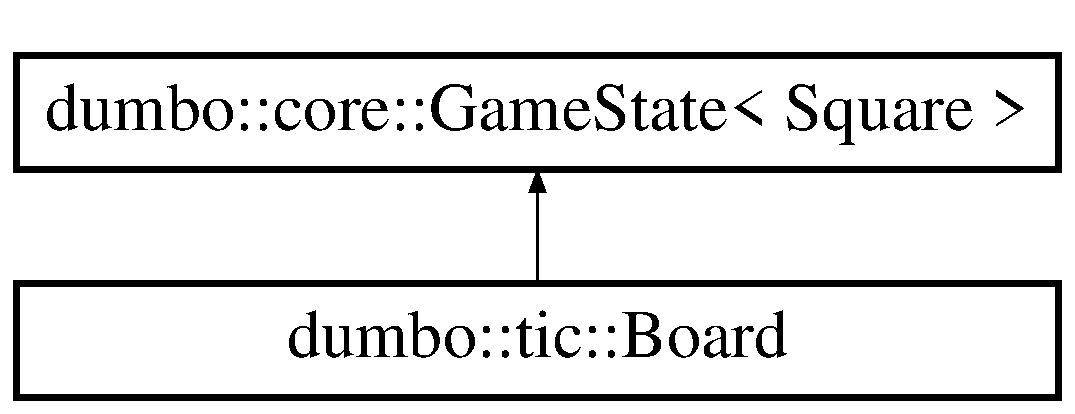
\includegraphics[height=2.000000cm]{classdumbo_1_1tic_1_1_board}
\end{center}
\end{figure}
\subsection*{Public Member Functions}
\begin{DoxyCompactItemize}
\item 
\hypertarget{classdumbo_1_1tic_1_1_board_a9b234c352e04139da4d375dcf0ce3d8e}{{\bfseries Board} (bool my\-\_\-turn=true)}\label{classdumbo_1_1tic_1_1_board_a9b234c352e04139da4d375dcf0ce3d8e}

\item 
\hypertarget{classdumbo_1_1tic_1_1_board_a1f37a5931e50d83527eba709dafc6ae5}{std\-::vector$<$ \hyperlink{structdumbo_1_1tic_1_1_square}{Square} $>$ {\bfseries Legal\-Moves} () const }\label{classdumbo_1_1tic_1_1_board_a1f37a5931e50d83527eba709dafc6ae5}

\item 
\hypertarget{classdumbo_1_1tic_1_1_board_a57b52e433e43323e558442dd09c6b7f2}{\hyperlink{structdumbo_1_1tic_1_1_square}{Square} {\bfseries Random\-Move} () const }\label{classdumbo_1_1tic_1_1_board_a57b52e433e43323e558442dd09c6b7f2}

\item 
\hypertarget{classdumbo_1_1tic_1_1_board_a7b362214b4e0018fd564298d44834e61}{bool {\bfseries Next\-State} (const \hyperlink{structdumbo_1_1tic_1_1_square}{Square} \&move, Game\-State $\ast$next\-\_\-state) const }\label{classdumbo_1_1tic_1_1_board_a7b362214b4e0018fd564298d44834e61}

\item 
\hypertarget{classdumbo_1_1tic_1_1_board_afcb179dde40eeef088cdda515da705cd}{bool {\bfseries Is\-Terminal} (double $\ast$win) const }\label{classdumbo_1_1tic_1_1_board_afcb179dde40eeef088cdda515da705cd}

\item 
\hypertarget{classdumbo_1_1tic_1_1_board_a380495a9e4113a5da8bc7ab927f37f60}{bool {\bfseries Is\-My\-Turn} () const }\label{classdumbo_1_1tic_1_1_board_a380495a9e4113a5da8bc7ab927f37f60}

\item 
\hypertarget{classdumbo_1_1tic_1_1_board_a5d5c5c7448d1451033a508486c72303b}{bool {\bfseries operator==} (const Game\-State$<$ \hyperlink{structdumbo_1_1tic_1_1_square}{Square} $>$ \&rhs) const }\label{classdumbo_1_1tic_1_1_board_a5d5c5c7448d1451033a508486c72303b}

\item 
\hypertarget{classdumbo_1_1tic_1_1_board_a844fcf752e4f9bcc2d2f43e1acbb22fe}{void {\bfseries Render} () const }\label{classdumbo_1_1tic_1_1_board_a844fcf752e4f9bcc2d2f43e1acbb22fe}

\end{DoxyCompactItemize}
\subsection*{Public Attributes}
\begin{DoxyCompactItemize}
\item 
{\bfseries my\-\_\-turn}
\end{DoxyCompactItemize}
\subsection*{Additional Inherited Members}


\subsection{Detailed Description}


Definition at line 56 of file board.\-h.



\subsection{Member Data Documentation}
\hypertarget{classdumbo_1_1tic_1_1_board_a1a2d7a8b6a19d97fabf37a51a31d9ff4}{\index{dumbo\-::tic\-::\-Board@{dumbo\-::tic\-::\-Board}!my\-\_\-turn@{my\-\_\-turn}}
\index{my\-\_\-turn@{my\-\_\-turn}!dumbo::tic::Board@{dumbo\-::tic\-::\-Board}}
\subsubsection[{my\-\_\-turn}]{\setlength{\rightskip}{0pt plus 5cm}dumbo\-::tic\-::\-Board\-::my\-\_\-turn}}\label{classdumbo_1_1tic_1_1_board_a1a2d7a8b6a19d97fabf37a51a31d9ff4}
{\bfseries Initial value\-:}
\begin{DoxyCode}
\{\}
  Board(\textcolor{keyword}{const} std::unordered\_set<Square, Square::Hasher>& occupied\_squares,
        \textcolor{keywordtype}{bool} my\_turn = \textcolor{keyword}{true})
\end{DoxyCode}


Definition at line 59 of file board.\-h.



The documentation for this class was generated from the following files\-:\begin{DoxyCompactItemize}
\item 
/home/travis/build/dfridovi/dumbo/include/dumbo/tic\-\_\-tac\-\_\-toe/board.\-h\item 
/home/travis/build/dfridovi/dumbo/src/tic\-\_\-tac\-\_\-toe/board.\-cpp\end{DoxyCompactItemize}

\hypertarget{classdumbo_1_1core_1_1_game_state}{\section{dumbo\-:\-:core\-:\-:Game\-State$<$ M $>$ Class Template Reference}
\label{classdumbo_1_1core_1_1_game_state}\index{dumbo\-::core\-::\-Game\-State$<$ M $>$@{dumbo\-::core\-::\-Game\-State$<$ M $>$}}
}
\subsection*{Public Member Functions}
\begin{DoxyCompactItemize}
\item 
\hypertarget{classdumbo_1_1core_1_1_game_state_a8b69e211496715e3969e5870df7428ae}{virtual std\-::vector$<$ M $>$ {\bfseries Legal\-Moves} () const =0}\label{classdumbo_1_1core_1_1_game_state_a8b69e211496715e3969e5870df7428ae}

\item 
\hypertarget{classdumbo_1_1core_1_1_game_state_aa23134e68598c061db73b70bfc968c35}{virtual M {\bfseries Random\-Move} () const =0}\label{classdumbo_1_1core_1_1_game_state_aa23134e68598c061db73b70bfc968c35}

\item 
\hypertarget{classdumbo_1_1core_1_1_game_state_a3e225cf3b0e9b396ae784612171c1035}{virtual bool {\bfseries Next\-State} (const M \&move, \hyperlink{classdumbo_1_1core_1_1_game_state}{Game\-State} $\ast$next\-\_\-state) const =0}\label{classdumbo_1_1core_1_1_game_state_a3e225cf3b0e9b396ae784612171c1035}

\item 
\hypertarget{classdumbo_1_1core_1_1_game_state_ac57f7f288be7ff5d1099fda47bb2e117}{virtual bool {\bfseries Is\-Terminal} (double $\ast$win) const =0}\label{classdumbo_1_1core_1_1_game_state_ac57f7f288be7ff5d1099fda47bb2e117}

\item 
\hypertarget{classdumbo_1_1core_1_1_game_state_ae89148286c9ae76017aec212efe393bd}{bool {\bfseries Is\-My\-Turn} () const }\label{classdumbo_1_1core_1_1_game_state_ae89148286c9ae76017aec212efe393bd}

\item 
\hypertarget{classdumbo_1_1core_1_1_game_state_ae244ca510aa640f97847fbaff6f2fa3d}{virtual bool {\bfseries operator==} (const \hyperlink{classdumbo_1_1core_1_1_game_state}{Game\-State}$<$ M $>$ \&rhs) const =0}\label{classdumbo_1_1core_1_1_game_state_ae244ca510aa640f97847fbaff6f2fa3d}

\item 
\hypertarget{classdumbo_1_1core_1_1_game_state_afad8470a5155a6a0c7ef244f1eb1ffac}{virtual void {\bfseries Render} () const =0}\label{classdumbo_1_1core_1_1_game_state_afad8470a5155a6a0c7ef244f1eb1ffac}

\end{DoxyCompactItemize}
\subsection*{Protected Member Functions}
\begin{DoxyCompactItemize}
\item 
\hypertarget{classdumbo_1_1core_1_1_game_state_a761603059309aba8469e98b9f6e517ec}{{\bfseries Game\-State} (bool my\-\_\-turn=true)}\label{classdumbo_1_1core_1_1_game_state_a761603059309aba8469e98b9f6e517ec}

\end{DoxyCompactItemize}
\subsection*{Protected Attributes}
\begin{DoxyCompactItemize}
\item 
\hypertarget{classdumbo_1_1core_1_1_game_state_af68aa1b2b5622077801b6fee2880828a}{bool {\bfseries my\-\_\-turn\-\_\-}}\label{classdumbo_1_1core_1_1_game_state_af68aa1b2b5622077801b6fee2880828a}

\end{DoxyCompactItemize}
\subsection*{Static Protected Attributes}
\begin{DoxyCompactItemize}
\item 
\hypertarget{classdumbo_1_1core_1_1_game_state_aafcc889dc70678e3a9840d1f8fd3805a}{static std\-::random\-\_\-device {\bfseries rd\-\_\-}}\label{classdumbo_1_1core_1_1_game_state_aafcc889dc70678e3a9840d1f8fd3805a}

\item 
\hypertarget{classdumbo_1_1core_1_1_game_state_a89930dde860d8e21e286106e2418609f}{static std\-::default\-\_\-random\-\_\-engine {\bfseries rng\-\_\-}}\label{classdumbo_1_1core_1_1_game_state_a89930dde860d8e21e286106e2418609f}

\end{DoxyCompactItemize}


\subsection{Detailed Description}
\subsubsection*{template$<$typename M$>$class dumbo\-::core\-::\-Game\-State$<$ M $>$}



Definition at line 55 of file game\-\_\-state.\-h.



The documentation for this class was generated from the following file\-:\begin{DoxyCompactItemize}
\item 
/home/travis/build/dfridovi/dumbo/include/dumbo/core/game\-\_\-state.\-h\end{DoxyCompactItemize}

\hypertarget{structdumbo_1_1tic_1_1_square_1_1_hasher}{\section{dumbo\-:\-:tic\-:\-:Square\-:\-:Hasher Struct Reference}
\label{structdumbo_1_1tic_1_1_square_1_1_hasher}\index{dumbo\-::tic\-::\-Square\-::\-Hasher@{dumbo\-::tic\-::\-Square\-::\-Hasher}}
}
\subsection*{Public Member Functions}
\begin{DoxyCompactItemize}
\item 
\hypertarget{structdumbo_1_1tic_1_1_square_1_1_hasher_ac82f53735d689a147db1bd0af659703e}{size\-\_\-t {\bfseries operator()} (const \hyperlink{structdumbo_1_1tic_1_1_square}{Square} \&sq) const }\label{structdumbo_1_1tic_1_1_square_1_1_hasher_ac82f53735d689a147db1bd0af659703e}

\end{DoxyCompactItemize}


\subsection{Detailed Description}


Definition at line 92 of file square.\-h.



The documentation for this struct was generated from the following file\-:\begin{DoxyCompactItemize}
\item 
/home/travis/build/dfridovi/dumbo/include/dumbo/tic\-\_\-tac\-\_\-toe/square.\-h\end{DoxyCompactItemize}

\hypertarget{classdumbo_1_1core_1_1_m_c_t_s}{\section{dumbo\-:\-:core\-:\-:M\-C\-T\-S$<$ M, G $>$ Class Template Reference}
\label{classdumbo_1_1core_1_1_m_c_t_s}\index{dumbo\-::core\-::\-M\-C\-T\-S$<$ M, G $>$@{dumbo\-::core\-::\-M\-C\-T\-S$<$ M, G $>$}}
}
Inheritance diagram for dumbo\-:\-:core\-:\-:M\-C\-T\-S$<$ M, G $>$\-:\begin{figure}[H]
\begin{center}
\leavevmode
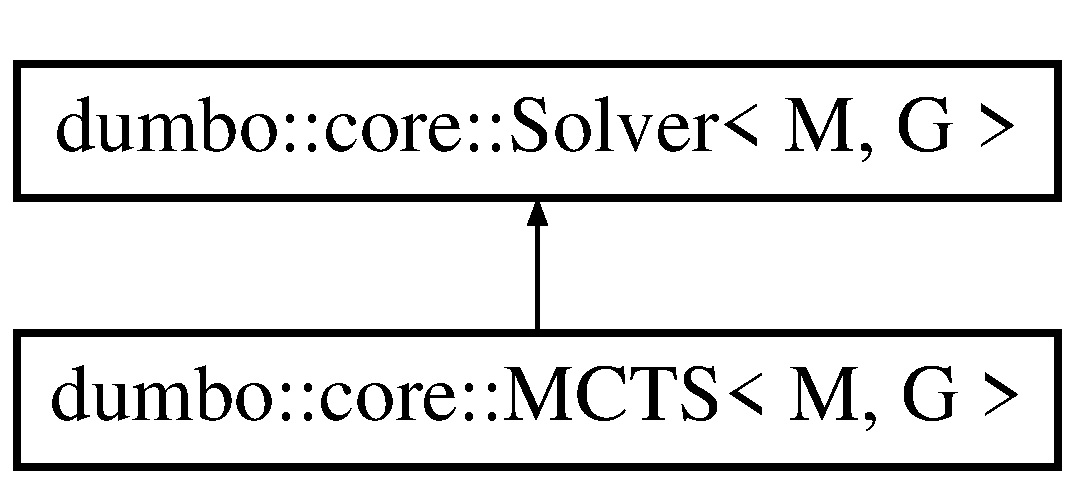
\includegraphics[height=2.000000cm]{classdumbo_1_1core_1_1_m_c_t_s}
\end{center}
\end{figure}
\subsection*{Public Member Functions}
\begin{DoxyCompactItemize}
\item 
\hypertarget{classdumbo_1_1core_1_1_m_c_t_s_adc54c1c87ffe8ceb3497847acae9a5b1}{{\bfseries M\-C\-T\-S} (double max\-\_\-time\-\_\-per\-\_\-move=1.\-0)}\label{classdumbo_1_1core_1_1_m_c_t_s_adc54c1c87ffe8ceb3497847acae9a5b1}

\item 
\hypertarget{classdumbo_1_1core_1_1_m_c_t_s_a2d62159e6a1d4c71a89fa81aa0d8dd93}{M {\bfseries Run} (const G \&state)}\label{classdumbo_1_1core_1_1_m_c_t_s_a2d62159e6a1d4c71a89fa81aa0d8dd93}

\end{DoxyCompactItemize}
\subsection*{Additional Inherited Members}


\subsection{Detailed Description}
\subsubsection*{template$<$typename M, typename G$>$class dumbo\-::core\-::\-M\-C\-T\-S$<$ M, G $>$}



Definition at line 62 of file mcts.\-h.



The documentation for this class was generated from the following file\-:\begin{DoxyCompactItemize}
\item 
/home/travis/build/dfridovi/dumbo/include/dumbo/core/mcts.\-h\end{DoxyCompactItemize}

\hypertarget{classdumbo_1_1core_1_1_move}{\section{dumbo\-:\-:core\-:\-:Move Class Reference}
\label{classdumbo_1_1core_1_1_move}\index{dumbo\-::core\-::\-Move@{dumbo\-::core\-::\-Move}}
}
Inheritance diagram for dumbo\-:\-:core\-:\-:Move\-:\begin{figure}[H]
\begin{center}
\leavevmode
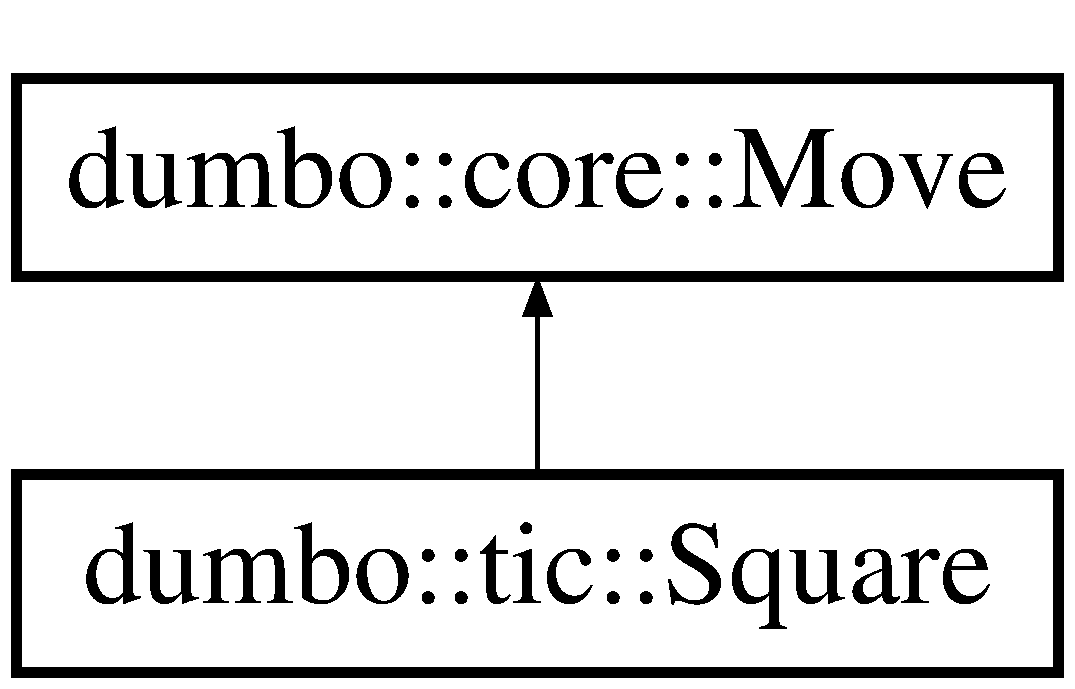
\includegraphics[height=2.000000cm]{classdumbo_1_1core_1_1_move}
\end{center}
\end{figure}
\subsection*{Protected Member Functions}
\begin{DoxyCompactItemize}
\item 
\hypertarget{classdumbo_1_1core_1_1_move_a9342b51029e64313ef79d443b8c31c20}{virtual void {\bfseries Print} (std\-::ostream \&output) const =0}\label{classdumbo_1_1core_1_1_move_a9342b51029e64313ef79d443b8c31c20}

\item 
\hypertarget{classdumbo_1_1core_1_1_move_aa7e93a65d69ca9f5ad22e2ee5a362411}{virtual void {\bfseries Load} (std\-::istream \&input)=0}\label{classdumbo_1_1core_1_1_move_aa7e93a65d69ca9f5ad22e2ee5a362411}

\end{DoxyCompactItemize}
\subsection*{Friends}
\begin{DoxyCompactItemize}
\item 
\hypertarget{classdumbo_1_1core_1_1_move_a1c86e73c26000947e25e7bc4b7f61b12}{std\-::ostream \& {\bfseries operator$<$$<$} (std\-::ostream \&output, const \hyperlink{classdumbo_1_1core_1_1_move}{Move} \&move)}\label{classdumbo_1_1core_1_1_move_a1c86e73c26000947e25e7bc4b7f61b12}

\item 
\hypertarget{classdumbo_1_1core_1_1_move_afa6f21808cceb074dc6bed218ee937e6}{std\-::istream \& {\bfseries operator$>$$>$} (std\-::istream \&input, \hyperlink{classdumbo_1_1core_1_1_move}{Move} \&move)}\label{classdumbo_1_1core_1_1_move_afa6f21808cceb074dc6bed218ee937e6}

\end{DoxyCompactItemize}


\subsection{Detailed Description}


Definition at line 51 of file move.\-h.



The documentation for this class was generated from the following file\-:\begin{DoxyCompactItemize}
\item 
/home/travis/build/dfridovi/dumbo/include/dumbo/core/move.\-h\end{DoxyCompactItemize}

\hypertarget{classdumbo_1_1core_1_1_player}{\section{dumbo\-:\-:core\-:\-:Player$<$ M, G $>$ Class Template Reference}
\label{classdumbo_1_1core_1_1_player}\index{dumbo\-::core\-::\-Player$<$ M, G $>$@{dumbo\-::core\-::\-Player$<$ M, G $>$}}
}
\subsection*{Public Member Functions}
\begin{DoxyCompactItemize}
\item 
\hypertarget{classdumbo_1_1core_1_1_player_ad9550ea94ab9036808b08adb19748bf1}{{\bfseries Player} (const G \&initial\-\_\-state, std\-::unique\-\_\-ptr$<$ \hyperlink{classdumbo_1_1core_1_1_solver}{Solver}$<$ M, G $>$$>$ solver)}\label{classdumbo_1_1core_1_1_player_ad9550ea94ab9036808b08adb19748bf1}

\item 
\hypertarget{classdumbo_1_1core_1_1_player_a5c645c33681a90afbed55ee3f97b6bb4}{void {\bfseries Play} ()}\label{classdumbo_1_1core_1_1_player_a5c645c33681a90afbed55ee3f97b6bb4}

\end{DoxyCompactItemize}


\subsection{Detailed Description}
\subsubsection*{template$<$typename M, typename G$>$class dumbo\-::core\-::\-Player$<$ M, G $>$}



Definition at line 59 of file player.\-h.



The documentation for this class was generated from the following file\-:\begin{DoxyCompactItemize}
\item 
/home/travis/build/dfridovi/dumbo/include/dumbo/core/player.\-h\end{DoxyCompactItemize}

\hypertarget{classdumbo_1_1core_1_1_solver}{\section{dumbo\-:\-:core\-:\-:Solver$<$ M, G $>$ Class Template Reference}
\label{classdumbo_1_1core_1_1_solver}\index{dumbo\-::core\-::\-Solver$<$ M, G $>$@{dumbo\-::core\-::\-Solver$<$ M, G $>$}}
}
Inheritance diagram for dumbo\-:\-:core\-:\-:Solver$<$ M, G $>$\-:\begin{figure}[H]
\begin{center}
\leavevmode
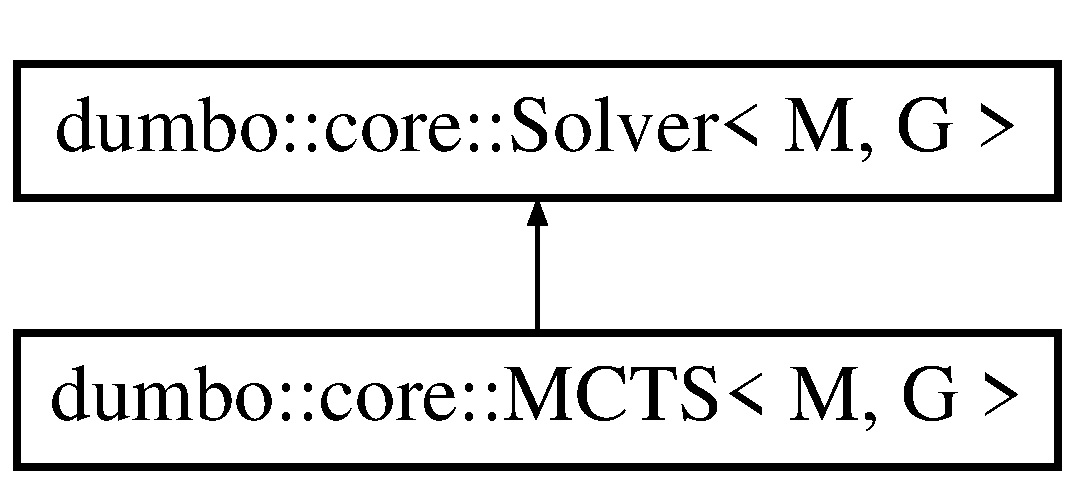
\includegraphics[height=2.000000cm]{classdumbo_1_1core_1_1_solver}
\end{center}
\end{figure}
\subsection*{Public Member Functions}
\begin{DoxyCompactItemize}
\item 
\hypertarget{classdumbo_1_1core_1_1_solver_a0ed80e080e6a47d31eccb4499317b951}{virtual M {\bfseries Run} (const G \&state)=0}\label{classdumbo_1_1core_1_1_solver_a0ed80e080e6a47d31eccb4499317b951}

\end{DoxyCompactItemize}
\subsection*{Protected Member Functions}
\begin{DoxyCompactItemize}
\item 
\hypertarget{classdumbo_1_1core_1_1_solver_a72cb33718fabd620575ea83b423a8892}{{\bfseries Solver} (double max\-\_\-time\-\_\-per\-\_\-move=1.\-0)}\label{classdumbo_1_1core_1_1_solver_a72cb33718fabd620575ea83b423a8892}

\end{DoxyCompactItemize}
\subsection*{Protected Attributes}
\begin{DoxyCompactItemize}
\item 
\hypertarget{classdumbo_1_1core_1_1_solver_a7da3faf09f70065d5f0928fe1f648cf9}{double {\bfseries max\-\_\-time\-\_\-per\-\_\-move\-\_\-}}\label{classdumbo_1_1core_1_1_solver_a7da3faf09f70065d5f0928fe1f648cf9}

\end{DoxyCompactItemize}


\subsection{Detailed Description}
\subsubsection*{template$<$typename M, typename G$>$class dumbo\-::core\-::\-Solver$<$ M, G $>$}



Definition at line 55 of file solver.\-h.



The documentation for this class was generated from the following file\-:\begin{DoxyCompactItemize}
\item 
/home/travis/build/dfridovi/dumbo/include/dumbo/core/solver.\-h\end{DoxyCompactItemize}

\hypertarget{structdumbo_1_1tic_1_1_square}{\section{dumbo\-:\-:tic\-:\-:Square Struct Reference}
\label{structdumbo_1_1tic_1_1_square}\index{dumbo\-::tic\-::\-Square@{dumbo\-::tic\-::\-Square}}
}
Inheritance diagram for dumbo\-:\-:tic\-:\-:Square\-:\begin{figure}[H]
\begin{center}
\leavevmode
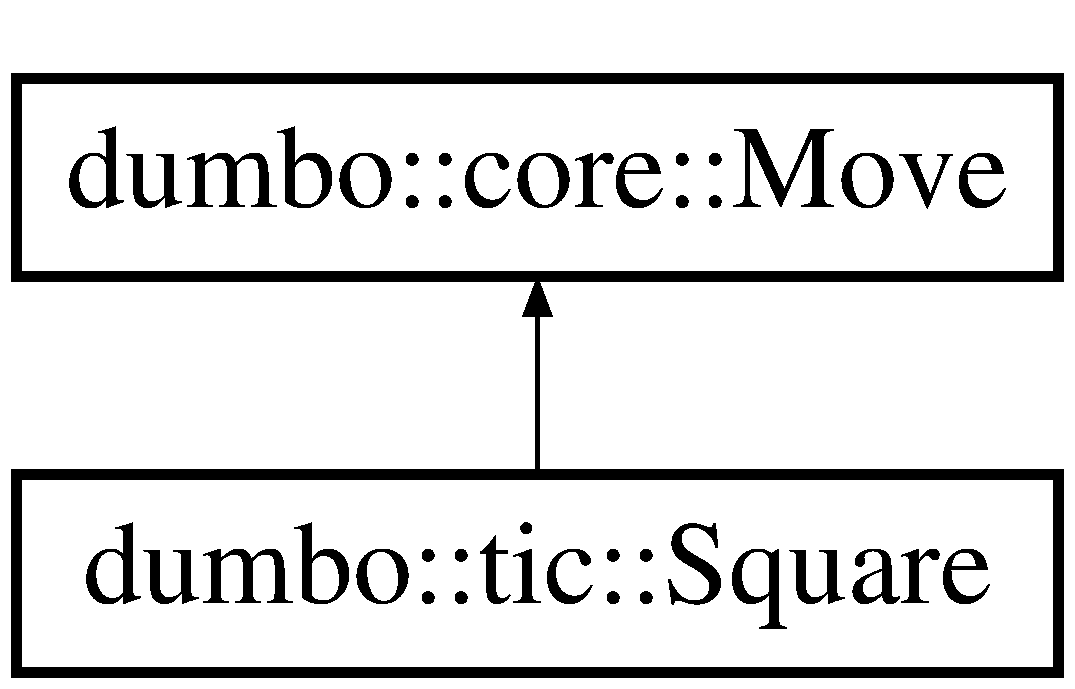
\includegraphics[height=2.000000cm]{structdumbo_1_1tic_1_1_square}
\end{center}
\end{figure}
\subsection*{Classes}
\begin{DoxyCompactItemize}
\item 
struct \hyperlink{structdumbo_1_1tic_1_1_square_1_1_hasher}{Hasher}
\end{DoxyCompactItemize}
\subsection*{Public Member Functions}
\begin{DoxyCompactItemize}
\item 
\hypertarget{structdumbo_1_1tic_1_1_square_ac6108c970f1a1967ecda40cf472493c3}{{\bfseries Square} (uint8\-\_\-t ii, uint8\-\_\-t jj, bool mine)}\label{structdumbo_1_1tic_1_1_square_ac6108c970f1a1967ecda40cf472493c3}

\item 
\hypertarget{structdumbo_1_1tic_1_1_square_aab8f80567a53c2c536115bcba0b0b6d2}{void {\bfseries Print} (std\-::ostream \&output) const }\label{structdumbo_1_1tic_1_1_square_aab8f80567a53c2c536115bcba0b0b6d2}

\item 
\hypertarget{structdumbo_1_1tic_1_1_square_a8677374ea58bcaf6968eed4146296a5b}{void {\bfseries Load} (std\-::istream \&input)}\label{structdumbo_1_1tic_1_1_square_a8677374ea58bcaf6968eed4146296a5b}

\item 
\hypertarget{structdumbo_1_1tic_1_1_square_a04ab41c06f16d672c03d8be122f3816d}{bool {\bfseries operator==} (const \hyperlink{structdumbo_1_1tic_1_1_square}{Square} \&rhs) const }\label{structdumbo_1_1tic_1_1_square_a04ab41c06f16d672c03d8be122f3816d}

\end{DoxyCompactItemize}
\subsection*{Public Attributes}
\begin{DoxyCompactItemize}
\item 
\hypertarget{structdumbo_1_1tic_1_1_square_a17fa8a9150e6a6e5dbc1fe0af4676666}{uint8\-\_\-t {\bfseries row} = 0}\label{structdumbo_1_1tic_1_1_square_a17fa8a9150e6a6e5dbc1fe0af4676666}

\item 
\hypertarget{structdumbo_1_1tic_1_1_square_a775434d24532f0ba45fcd35b0323639e}{uint8\-\_\-t {\bfseries col} = 0}\label{structdumbo_1_1tic_1_1_square_a775434d24532f0ba45fcd35b0323639e}

\item 
\hypertarget{structdumbo_1_1tic_1_1_square_a64e4349404fa0476ea44c8b52986d0e6}{bool {\bfseries my\-\_\-square} = true}\label{structdumbo_1_1tic_1_1_square_a64e4349404fa0476ea44c8b52986d0e6}

\end{DoxyCompactItemize}
\subsection*{Additional Inherited Members}


\subsection{Detailed Description}


Definition at line 56 of file square.\-h.



The documentation for this struct was generated from the following file\-:\begin{DoxyCompactItemize}
\item 
/home/travis/build/dfridovi/dumbo/include/dumbo/tic\-\_\-tac\-\_\-toe/square.\-h\end{DoxyCompactItemize}

%--- End generated contents ---

% Index
\newpage
\phantomsection
\addcontentsline{toc}{chapter}{Index}
\printindex

\end{document}
